\chapter{Quarto Projeto: Sistema para Locação de Mídias}\label{cap:quartoProjeto}
\epigraph{``\textit{Com organização e tempo, acha-se o segredo de fazer tudo e bem feito}''.}{Pitágoras}

\lettrine[lines=4, lhang=0.1, lraise=0, loversize=0.2, findent=0.1em]{\textcolor{corAzulTema}{N}}{ESTE} Capítulo aplicaremos o conhecimento adquirido até o momento na construção de uma aplicação Web em Java totalmente funcional, terminando o desenvolvimento do sistema de locação de DVDs começado no Capítulo~\ref{cap:segundoProjeto}, alterando diversas coisas que já foram feitas, inserindo a possibilidade do cadastro de mídias de vários tipos e, enfim, a locação de um ou mais mídias por cada cliente. Sim, eu sei que locadora de DVDs, BluRays etc. não são mais tão populares, mas acredito que você saiba o que são e é um bom exemplo para podermos colocar o que sabemos em prática.


\section{Introdução}

Assim como no Capítulo~\ref{cap:segundoProjeto}, neste Capítulo será apresentada uma série de requisitos que devem ser usados para criar uma aplicação Web da mesma forma que fizemos no Capítulo~\ref{cap:terceiroProjeto}. Novamente, tudo que será requisitado estará baseado no que já aprendemos, sendo assim, todas as funcionalidades requeridas poderão ser implementadas com recursos já vistos no Capítulo~\ref{cap:terceiroProjeto}. Agora você está apto a desenvolver um sistema completo de locação de mídias usando tudo que aprendeu até o momento. Vamos lá?


\section{Apresentação dos Requisitos}

Você foi contratado para criar um sistema para controle de cadastro de mídias. Esse sistema irá manter o cadastro dessas mídias e permitirá que clientes as aluguem. O diagrama do modelo físico do banco de dados pode ser visto na Figura~\ref{fig:cap09ModeloFisico}. Para gerar a base, com o MariaDB/MySQL em execução, abra o modelo da base no MySQL Workbench, disponibilizado nos arquivos do Capítulo.

\FloatBarrier
\begin{figure}[!htbp]
    \centering
    \caption{Diagrama do modelo físico da base de dados}
    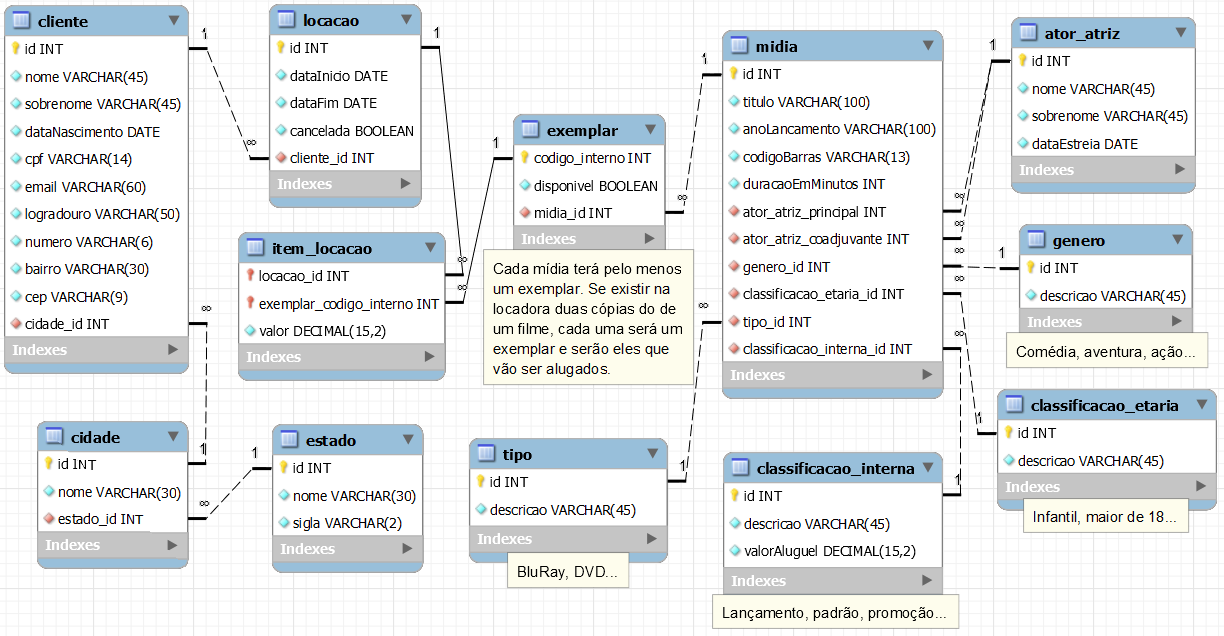
\includegraphics[scale=0.5]{imagens/cap09ModeloFisico}
    \\\textbf{Fonte:} Elaborada pelo autor
    \label{fig:cap09ModeloFisico}
\end{figure}
\FloatBarrier

As entidades e seus atributos você poderá ver no diagrama apresentado acima. Abaixo serão explicados os detalhes de cada uma das funcionalidades. Cada um dos cadastros base, ou seja, cadastro de mídias e seus exemplares, atores/atrizes, gêneros, classificações etárias, tipos, classificações internas, clientes, cidades e estados, deve conter as funcionalidades de criar, alterar e excluir um determinado registro. A página principal da aplicação deve conter um link para cada tipo de cadastro. Cada mídia pode ter um ou mais de um exemplares. O valor da locação virá da classificação interna de uma mídia, por exemplo, quando um filme ou jogo é lançamento, a locação é mais cara, concorda? Abaixo de cada nova tabela há uma caixa de texto com alguns exemplos do que poderia haver naquele cadastro para que você possa se guiar. O processo de locação é análogo ao processo de venda de produtos do Capítulo~\ref{cap:terceiroProjeto} e aqui a locação é por exemplar, então a tabela de itens de locação já está correta para a modelagem da solução desse problema.


\section{Desenvolvimento do Projeto}

O projeto Web que deverá ser criado deve ter o nome de ``LocacaoMidias''. Configure o projeto para conter as bibliotecas internamente. O pacote de código-fonte base do projeto deve ter o nome de ``\texttt{locacaomidias}''. A estrutura do projeto deve ser igual à estrutura do projeto criado no Capítulo~\ref{cap:terceiroProjeto}, sendo que, obviamente, o nome das classes e suas respectivas implementações serão diferentes do projeto daquele Capítulo. A base de dados com as tabelas das entidades obtidas a partir da análise dos requisitos na seção anterior deve ter o nome de ``\texttt{locacao\_midias}''. Não se esqueça de que cada entidade deverá conter um identificador. As páginas da aplicação deverão ter sua aparência configurada usando uma folha de estilos, da mesma forma que fizemos no projeto do Capítulo~\ref{cap:terceiroProjeto}. Nesse projeto você precisa obrigatoriamente trabalhar na aparência do sistema, criando um menu, usando imagens etc. ou seja, agora além de toda a implementação você precisará usar imagens ou quaisquer outros artifícios que julgar interessante para mudar a aparência da sua aplicação.


\section{Resumo}

Neste Capítulo foi requisitado que você implementasse uma aplicação Web em Java para gerenciar a locação de mídias como DVDs e BluRays, por isso, não há atividades a serem realizadas.
